% The 1 km pit, the 900 m rope and the knife — Geometry 30 of the abacus.
%
% Has words in it, so it is built twice: tools/build_figures.py passes
% \figlangru or \figlangen and \lang{…}{…} picks. Same rules as the other
% drawings: strokes black (rewritten to currentColor), fills mid-tone, no
% transparency.
\documentclass[tikz,dvisvgm,border=3pt]{standalone}
% T2A last, so it is the default: it carries Cyrillic *and* Latin, which is what
% lets one source set both languages.
\usepackage[T1,T2A]{fontenc}
\usepackage[utf8]{inputenc}
\usetikzlibrary{decorations.pathmorphing}

\newcommand{\lang}[2]{\ifdefined\figlangru#1\else#2\fi}

\definecolor{soil}{HTML}{A89377}
\definecolor{soildark}{HTML}{85735C}
\definecolor{rope}{HTML}{D08A2C}
\definecolor{steel}{HTML}{9BA3AE}
\definecolor{handle}{HTML}{6B4A2F}

\begin{document}
% 1 unit of y = 100 m of depth. The shaft is drawn narrow on purpose.
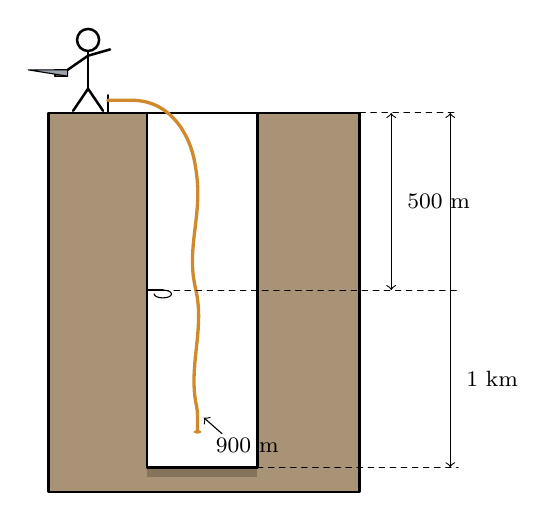
\begin{tikzpicture}[
  x=1cm, y=0.45cm,
  line join=round, line cap=round,
  edge/.style={line width=0.9pt},
  ropeline/.style={line width=1.2pt},
  thin_/.style={line width=0.4pt},
  lbl/.style={font=\footnotesize},
]

% ── the ground, cut open ──────────────────────────────────────────────────
\fill[soil] (-1.25,0) rectangle (0,-10.7);
\fill[soil] (1.4,0) rectangle (2.7,-10.7);
\fill[soil] (0,-10) rectangle (1.4,-10.7);
\fill[soildark] (0,-10) rectangle (1.4,-10.28);   % the floor of the shaft

\draw[edge] (-1.25,0) -- (0,0) -- (0,-10) -- (1.4,-10) -- (1.4,0) -- (2.7,0);
\draw[edge] (-1.25,-10.7) rectangle (2.7,0);

% ── the peg at the top and the hook halfway down ──────────────────────────
\draw[edge] (-0.5,0) -- (-0.5,0.5);
\draw[edge] (0,-5) -- (0.2,-5);
\draw[thin_] (0.2,-5) arc (90:-180:0.11);

% ── the rope: tied to the peg, 900 m of it, hanging 100 m short ───────────
\draw[ropeline, rope, rounded corners=1.5pt]
  (-0.5,0.36) -- (-0.2,0.36) .. controls (0.3,0.3) and (0.55,-0.6) ..
  (0.62,-1.6) .. controls (0.7,-2.9) and (0.5,-3.8) .. (0.62,-5)
  .. controls (0.72,-6.2) and (0.52,-7.2) .. (0.64,-8.4) -- (0.64,-9);
\fill[rope] (0.64,-9) circle (0.05);

% ── the climber, with the knife ───────────────────────────────────────────
\begin{scope}[shift={(-0.75,0.06)}, x=1cm, y=1cm, line width=0.9pt]
  \draw (0,0.28) -- (0,0.76);                    % body
  \fill[white] (0,0.9) circle (0.14);
  \draw (0,0.9) circle (0.14);                   % head
  \draw (0,0.7) -- (-0.26,0.52);                 % arm holding the knife
  \draw (0,0.7) -- (0.28,0.78);                  % arm pointing at the pit
  \draw (0,0.28) -- (-0.19,0);                   % legs
  \draw (0,0.28) -- (0.19,0);
  % the knife, in the lowered hand
  \fill[handle] (-0.42,0.44) rectangle (-0.26,0.52);
  \draw[line width=0.4pt] (-0.42,0.44) rectangle (-0.26,0.52);
  \fill[steel] (-0.26,0.44) -- (-0.26,0.52) -- (-0.76,0.52) -- cycle;
  \draw[line width=0.4pt] (-0.26,0.44) -- (-0.26,0.52) -- (-0.76,0.52) -- cycle;
\end{scope}

% ── measurements, kept clear of the earth ─────────────────────────────────
\draw[thin_, dash pattern=on 2pt off 2pt] (0.2,-5) -- (3.95,-5);
\draw[thin_, dash pattern=on 2pt off 2pt] (1.4,-10) -- (3.95,-10);
\draw[thin_, dash pattern=on 2pt off 2pt] (2.7,0) -- (3.95,0);

\draw[thin_, <->] (3.1,0) -- (3.1,-5);
\node[lbl, anchor=west] at (3.18,-2.5) {\lang{500 м}{500 m}};

\draw[thin_, <->] (3.85,0) -- (3.85,-10);
\node[lbl, anchor=west] at (3.93,-7.5) {\lang{1 км}{1 km}};

\node[lbl, anchor=north west] at (0.75,-8.9) {\lang{900 м}{900 m}};
\draw[thin_, ->] (0.95,-9.05) -- (0.72,-8.6);

\end{tikzpicture}
\end{document}
